\newpage % sonst formatierung im arsch 
\subsection{Aufagbenteil b, analog zu a was orga betrifft}
\label{sec:aufgabe_b}

Die Hallspannung ist grundelegend von zwei Werten abhängig. Dem \textbf{Magnetfeld} und der Spannung  $\symup{I_b}$ die den Elektronen eine Geschwindigkeit $v$ gibt, senkrecht zum Magnetfeld. %eventuell Verweise
Im folgen haben wir jeweils einen Wert konstant bei maximaler Spannung gehalten, für möglichst aussagenede Ergebnisse, und das Verhalten jeweils untersucht. 
Zudem differenzieren wir zwischen postiver und nagativer Polung um Messungenauigkeiten die den geräten verschuldet sind dadurch im späteren Verlauf auszuschlißen. % mehr Gründe hier.
Wir finden also zwei Abbildung, die sich sehr ähnlich sind. Für den genauen Wert der Spannung bedienen wir uns anschließedn dem Zusammenhang \cite[9]{V311.pdf} 

\begin{align*}
\symup{U_{ges+}}&= \symup{U_{h}} + \symup{U_{stör}} \\
\symup{U_{ges-}}&= - \symup{U_{h}} + \symup{U_{stör}} \\
\end{align*}
\begin{equation}
\symup{U_{H}}= \frac{1}{2}(\symup{U_{ges+}} -\symup{U_{ges-}}
\end{equation}

Sowohl $\symup{U_{ges+}}$ als auch $\symup{U_{ges-}}$ ist uns als Messung und als Graph bekannt, also könenn wir nun die finale Hallspannung sowhol 
ausrechnen als auch darstellen.


\subsubsection{konstantes Magnetfeld}
\label{sec:Auswertung_bconst}
Die ersten Messungen wurden mit konstantem Magnetfeld durch geführt. In unserem Fall lag der Strom $\symup{I_b}$, welcher den Elektromagneten betrieben hat bei konstanten $4.6\si{\ampere}$.
Der variable Teil kommt also durch den Strom $\symup{I_q}$ hinzu welcher bei $0\si{\ampere}$ beginnt und von uns vor jeder neuen Messung um $0.5\si{\ampere}$ erhöt wurde.
\\ %komisches layout von lateX, kp was da los ist
\begin{figure}[!h]
   \centering
    \includegraphics[width=\textwidth]{"build/u_hall.pdf"}
    \caption{iq variabel, Bfeld const\\Fehler für mT $\pm$ 0.0005\\Fehler für $I_b \pm 0.001$}
    \label{fig:Uhall}
\end{figure}

Der Graph wird durch ein Polynom dritten Grades dargestellt, verläuft aber annährend linear in beiden Pohl Richtungen. Auffallend ist die verschiebung auf der Y-Achse %Grund 
welche keinen Physikalischen Hintergrund hat. Also lässt sich diese als Fehler bewerten und gilt zu zukünftiger beachtung in kommenden Rechnungen.
Die verschiebung lässt sich errechnen in dem man die Werte für $\symup{I_b}=0$ des Polynoms sucht, welches durch folgende Parameter und Funktion gegeben wird.
\paragraph{positive Polung}

\begin{align*}
   &a = -0.000006 &&(\pm 0) \\
   &b = 0.000112 &&(\pm 0.0003)\\
   &c = 0.001876 &&(\pm 0.0006) \\
   &d = 0.000727 &&(\pm 0.0003) 
\end{align*}

\begin{equation}
   \symup{U_{ges+}}(\symup{I_q})=-0.000006 \cdot \symup{I_q}^3 + 0.000112\cdot\symup{I_q}^2 + 0.001876 \cdot\symup{I_q} + 0.000727 
\end{equation}

\paragraph{negative Polung} 

\begin{align*}
   &a = -0.000047 &&(\pm 0.0000) \\
   &b = 0.000280 &&(\pm 0.0001 ) \\
   &c = -0.002408 &&(\pm 0.0003) \\
   &d = 0.000084 &&(\pm 0.0002 ) 
\end{align*}
 
\begin{equation}
   \symup{U_{ges-}}(\symup{I_q})=-(-0.000047 \cdot \symup{I_q}^3 + 0.000280\cdot\symup{I_q}^2 -0.002408\cdot\symup{I_q} + 0.000084)
\end{equation}

%Die Nullstelle für den verschobenen Part der postiven Polung lässt durch einsetzten von $0$ bestimmen und sieht wie folgt aus:
%
%\begin{align}
%   \symup{m\si{\tesla}}(0)&=-0.000006 \cdot 0^3 + 0.000112 \cdot 0^2 + 0.001876 \cdot 0 + 0.000727 \\
%   \symup{m\si{\tesla}}(0)&=0.000727
%\end{align}
%
%Der Graph ist also um $0.000727$ $\symup{\si{\volt}}$ nach oben verschoben.
%Was in der Auswertung und berechnung von anderen Werten berücksichtigt werden muss.









\subsubsection{konstanter Strom $\symup{I_q}$}
\label{sec:Auswertung_iconst}

Diese abbildene Kurve der \textbf{Hallspannung} steht in Abhängigkeit zum Strom $\symup{I_b}$ der durch den Elektromagneten fließt und somit ein Magnetfeld erzeugt.
Der Graph ist deutlich stärker Gekrümmt als \ref{fig:Uhall} und wird wieder durch ein Poylnom dritten Grades abgebildet. 


\begin{figure}
   \centering
    \includegraphics[width=\textwidth]{"build/u_hall_i.pdf"}
    \caption{iq const, Bfeld variabelt$\pm$ 0.0005\\Fehler für $I_b \pm 0.001$}
    \label{fig:Uhall}
 \end{figure}



Dieses mal mit Parametern und Funktion analog zu \ref{sec:Auswertung_bconst}
\paragraph{Postive Polung}

\begin{align*}
&a = -0.000146 &&(\pm  0.0001) \\
&b = 0.001047 &&(\pm  0.0004 ) \\
&c = -0.000053 &&(\pm  0.0008) \\
&d = -0.000740 &&(\pm  0.0004) 
\end{align*}

\begin{equation}
   \symup{U_h}(\symup{I_b})=-0.000146 \cdot \symup{I_b}^3 + 0.001047\cdot\symup{I_b}^2 -0.000053\cdot\symup{I_b} -0.000740
\end{equation}

\paragraph{negaitve Polung}

\begin{align*}
&a = -0.000044 &&(\pm 0.0000) \\
&b = 0.000415 &&(\pm 0.0002) \\
&c = -0.003241 &&(\pm 0.0004) \\
&d = 0.000137 &&(\pm 0.0002) 
\end{align*}

\begin{equation}
   \symup{U_h}(\symup{I_b})=-0.000044 \cdot \symup{I_b}^3 + 0.000415\cdot\symup{I_b}^2 -0.003241\cdot\symup{I_b} 0.000137
\end{equation}

Es liegen uns also jetzt beide Auswertungen $\symup{U_{ges+}}$ und $\symup{U_{ges-}}$ die wir als folgende Darstellung abbilden können.
Man erkennt, dass die Spannung nahezun Exponentiell zum Magnetfeld ansteigt % was leider nicht passt lol... !!!!!!!!!!!!!

\begin{figure}
   \centering
   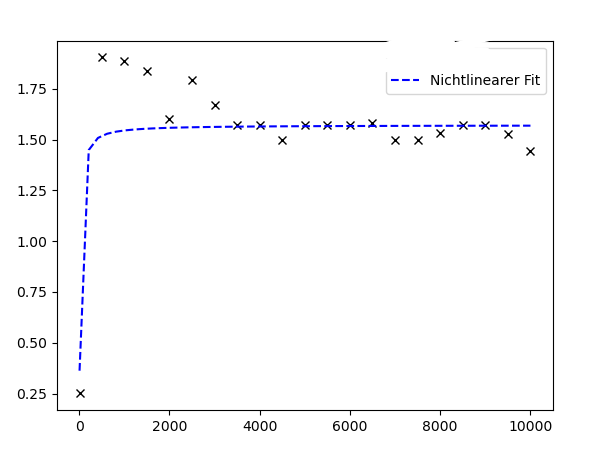
\includegraphics[width=\textwidth]{build/plot1.pdf}
   \caption{$\symup{U_h}$ als Überschneidung beider Pole}
   \label{fig:auswertunghall}
\end{figure}

Hier wird noch kein Fehler mit einbezogen, der durch die Messung entstanden ist. man kann den graphen bloß als eine art Annährung werten. 
Es beiet sich an mit Python den Fehler jeweils für die gemessenen Werte ausrechnen zu lassen und als Tabelle auszugeben.

%Tabelle mit weerten aus ugesamt 
%\begin{tabel}
%
%\end{tabel}